\documentclass[preprint,12pt]{elsarticle}
\myfooterfont{\scriptsize\itshape}
\makeatletter
\patchcmd{\ps@pprintTitle}
  {\hbox to \textwidth}
  {\hbox to \dimexpr\textwidth-3pt\relax}
  {}{}
\makeatother

\usepackage{amsmath,amssymb}
\usepackage{booktabs}
\usepackage{graphicx}
\usepackage{float}
\usepackage{siunitx}
\usepackage{xcolor}
\usepackage[hidelinks]{hyperref}
\usepackage{lineno}

% Keep full-width figures close to the discussion without creating sparse
% figure-only pages in the one-column review manuscript.
\setcounter{topnumber}{2}
\setcounter{bottomnumber}{1}
\setcounter{totalnumber}{3}
\renewcommand{\topfraction}{0.95}
\renewcommand{\bottomfraction}{0.80}
\renewcommand{\textfraction}{0.05}
\renewcommand{\floatpagefraction}{0.75}
\makeatletter
\setlength{\@fptop}{0pt}
\setlength{\@fpbot}{0pt plus 1fil}
\makeatother

\makeatletter
\pdfstringdefDisableCommands{%
  \def\corref#1{}%
  \def\cormark[#1]{}%
  \def\cnotenum{}%
  \def\@corref{}%
}
\makeatother

% Generated by code/build_hccb_p418_manuscript_values.py
\newcommand{\CompletedSteadyCases}{60}
\newcommand{\TotalSteadyCases}{60}
\newcommand{\SteadyProgressText}{60/60}
\newcommand{\RegionalNodes}{46089}
\newcommand{\RegionalEdges}{245848}
\newcommand{\TransientTimePoints}{56}
\newcommand{\TransientModelParameters}{270121}
\newcommand{\TransientPeakGpuGB}{18.99}
\newcommand{\InterfacePairCount}{513310}
\newcommand{\InterfaceFluxRelativeMismatch}{2.08\times 10^{-13}}
\newcommand{\MeshPorosity}{0.386791}
\newcommand{\LocalFlowCrossingMin}{0.0059}
\newcommand{\LocalFlowCrossingMax}{0.0293}
\newcommand{\ParticleConductionMin}{0.408}
\newcommand{\ParticleConductionMax}{0.593}

% Generated by code/build_hccb_p418_inlet_dimensionless_envelope.py
\newcommand{\InletReMin}{0.078}
\newcommand{\InletReMax}{2.40}
\newcommand{\InletPrMin}{0.660}
\newcommand{\InletPrMax}{0.675}
\newcommand{\InletPeMin}{0.051}
\newcommand{\InletPeMax}{1.62}
\newcommand{\HighInletReCaseCount}{6}


\newcommand{\LiSi}{Li$_4$SiO$_4$}
\newcommand{\OpenFOAM}{OpenFOAM}
\journal{International Journal of Heat and Mass Transfer}
\hypersetup{
  pdftitle={Transient conjugate heat transfer in internally heated ceramic pebble beds: pore-resolved reference fields and graph--Transformer prediction},
  pdfauthor={Jian Wang; Wei Wen; Gang Shen; Mingzhun Lei; Yuntao Song},
  pdfkeywords={solid-breeder blanket; ceramic pebble bed; conjugate heat transfer; physics-informed neural network; graph Transformer; diffusion refinement}
}

\begin{document}
\begin{frontmatter}

\title{Transient conjugate heat transfer in internally heated ceramic pebble beds: pore-resolved reference fields and graph--Transformer prediction}

\author[a,b]{Jian Wang\corref{cor1}}
\ead{wjfttt@mail.ustc.edu.cn}
\author[a,b]{Wei Wen}
\author[a]{Gang Shen}
\author[b]{Mingzhun Lei}
\author[b]{Yuntao Song}
\cortext[cor1]{Corresponding author.}

\address[a]{Anhui University of Science and Technology, Huainan 232001, China}
\address[b]{Institute of Plasma Physics, Hefei Institutes of Physical Science, Chinese Academy of Sciences, Hefei 230031, China}

\begin{abstract}
\IfFileExists{generated_final_abstract.tex}{\input{generated_final_abstract}}{%
Pore-scale heat transfer in solid-breeder pebble beds couples temperature-dependent helium flow, ceramic conduction, fluid--solid exchange, volumetric heating and wall cooling. Direct three-dimensional calculations resolve these mechanisms but are too expensive for repeated operating-condition and transient studies. We establish a pore-resolved benchmark and a hybrid prediction chain in which, at inference, a frozen steady coordinate PINN supplies the source-condition temperature and target-condition hydrodynamic state, a regional graph--Transformer predicts the fluid and solid temperature trajectory, and a diffusion-style refiner acts only on the remaining temperature error. Physics-constrained variants incorporate finite-volume mass, energy and interface heat-flux relations; all models are evaluated using the same physical quantities. Complete operating conditions and thermal-step trajectories are separated between training, validation and independent prediction. The database contains 60 steady conjugate-heat-transfer conditions and 12 fixed-hydrodynamics (hereafter fixed-flow) thermal-step trajectories. The regional representation contains \RegionalNodes{} nodes and \RegionalEdges{} connections, with \TransientTimePoints{} retained field times per trajectory. A second independently generated spherical-pebble arrangement was calculated at nine matched conditions. Relative to the reference arrangement, its outlet-temperature and maximum-solid-temperature changes remain below 0.67\% and 0.31\%, respectively, whereas the pressure-drop change is 14.7--18.0\%. For these two intact spherical arrangements, integral thermal response is therefore less packing-sensitive than hydraulic resistance. The final comparison tests whether the hybrid model accelerates the three-dimensional reference calculation while retaining hotspot magnitude and location, signed wall heat transfer and finite-volume energy consistency.
}
\end{abstract}

\begin{keyword}
solid-breeder blanket \sep ceramic pebble bed \sep conjugate heat transfer \sep physics-informed neural network \sep graph Transformer \sep diffusion refinement
\end{keyword}

\end{frontmatter}

\linenumbers

\section{Introduction}

Ceramic pebble beds in solid-breeder fusion blankets must remove internally
generated heat while maintaining temperatures suitable for tritium production
and release. Their response couples conduction in the ceramic, helium
advection and conduction, fluid--solid heat exchange, near-wall packing
structure and cooling-wall conditions. Experiments show that the effective
thermal conductivity of \LiSi{} and Li$_2$TiO$_3$ beds varies with temperature,
gas pressure, packing state and fabrication route
\cite{wang2020conductivity,patel2021hotwire,pupeschi2019thermal}. DEM studies
further show persistent wall-induced porosity oscillations and anisotropic
contact networks in confined breeder beds
\cite{gong2017hccbpacking,wang2021anisotropic}. Crushable-DEM calculations
add a further structural mechanism: compression-driven fragmentation changes
the particle-size distribution and the spatial pattern of crushing events,
implying possible changes in the contact topology relevant to heat transfer
\cite{wang2026crushable}. Effective-property models are
therefore essential for component calculations, and recent correlations span
particle--fluid heat transfer from laminar to turbulent flow in spherical
packed beds \cite{wu2025particlefluid}. They cannot, however, directly describe
preferential pore flow, local conjugate heat exchange or the position of a
solid hotspot.

Particle-resolved CFD provides this local information. For a Li$_2$TiO$_3$
canister, resolved and porous-medium models predicted similar mean outlet
temperatures, whereas only the resolved calculation exposed bypass flow and
inlet--outlet short-circuiting \cite{sharma2020purge}. Recent HCCB calculations
resolved helium flow and conjugate heat transfer under volumetric pebble
heating and used the resulting fields to examine macroscopic transport
\cite{wang2023pore,wang2024macro}. Repeating such calculations over velocity,
inlet-temperature, heat-source, packing and transient variations is
computationally expensive. A useful reduced model must consequently preserve
more than the outlet average: fluid and solid temperature fields, hotspot
magnitude and position, pressure drop, cooling-wall heat transfer and the
finite-volume mass and energy relations all remain relevant.

Physics-informed and operator-learning methods offer possible routes to this
reduction. Coordinate PINNs have inferred permeability, conductivity and
diffusion characteristics from breeder-bed fields
\cite{wang2024hccb_pinn,wang2025packed_diffusion_pinn}. Porous-DeepONet and
constraint-incorporated U-Nets encode porous structure on regular
representations \cite{huang2024porousdeeponet,guo2024constraintporous}, while a
finite-volume UNO-PINO imposes interfacial flux continuity and local
conservation for discontinuous two-phase conduction \cite{zhu2026unopino}.
Thermal PINNs also treat transient conduction, parameterized convection,
multi-domain conjugate heat transfer and hidden temperatures in porous flow
\cite{li2025improvedpinn,cui2025parameterizedpinn,lee2025empinn,
jang2026porousthermalpinn}.
Graph operators retain unstructured connectivity
\cite{pfaff2021meshgraphnets,mousavi2025rigno}, and attention-based mesh
operators add long-range and temporal coupling
\cite{wu2024transolver,garnier2026spatiotemporal,iparraguirre2026mgnt}.
Their value for an internally heated fluid--solid pebble bed has not been
tested on complete unseen conditions and trajectories, a different packing,
and common finite-volume measures.

We combine graph message passing, temporal attention and finite-volume
balances for transient pebble-bed heat transfer. The reference set contains
60 pore-resolved steady conditions, 12 fixed-hydrodynamics thermal steps and
nine matched calculations on an independent spherical packing. At inference,
a frozen coordinate PINN supplies endpoint fields, a graph--Transformer
advances both phase temperatures, and a diffusion-style model refines the
remaining temperature error. All baselines use identical condition and
trajectory splits. We test whether added complexity improves unseen fields
without degrading wall heat or energy consistency.

\begin{figure}[H]
\centering
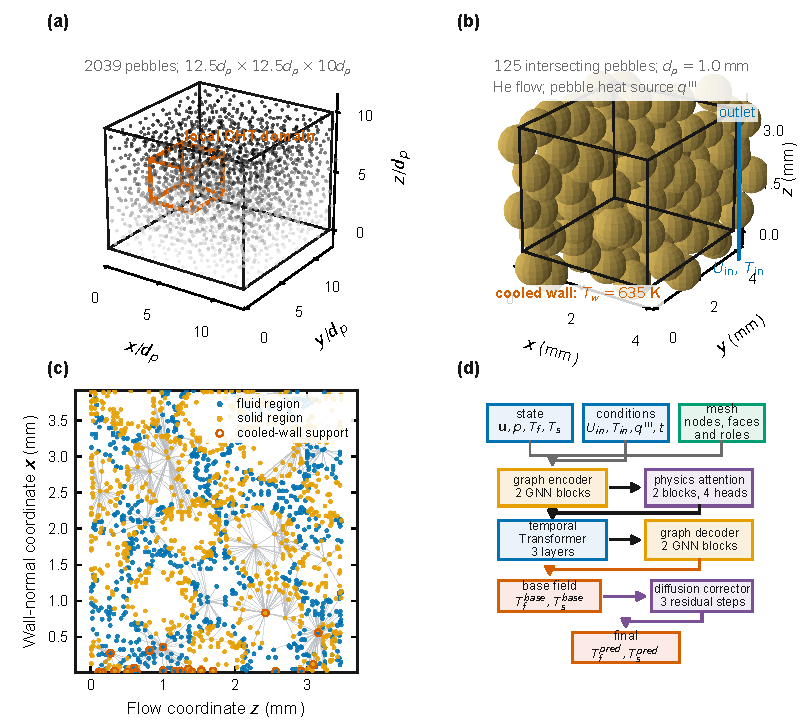
\includegraphics[width=\textwidth]{../figures/hccb_p418_physical_model_domain.pdf}
\caption{Physical domain and hybrid temperature model. (a) The 2039-pebble seed101 parent packing. (b) The resolved 125-pebble crop with helium flow, wall cooling and solid heating. (c) Fluid, solid and cooled-wall nodes in the 46\,089-node graph. (d) Local message passing, Physics-Attention and temporal Transformer produce the base temperature trajectory; the optional diffusion module refines only its temperature residual.}
\label{fig:workflow}
\end{figure}

\section{Methods}

\subsection{Reference problem and calculations}

The reference problem follows the published low-Reynolds-number HCCB
pore-scale configuration \cite{wang2023pore,wang2024macro}. Sixty steady
conditions combine five inlet velocities
(\SIrange{0.05}{0.25}{m.s^{-1}}), four inlet temperatures
(\SIrange{300}{900}{K}) and three pebble heat-source levels
(4.85, 6.85 and \SI{8.85}{MW.m^{-3}}). The outlet absolute pressure is
\SI{0.12}{MPa}, the cooled wall is held at \SI{635}{K}, and the spherical
\LiSi{} pebbles have a physical diameter of \SI{1}{mm}. At the inlet,
$Re_{p,\mathrm{in}}=0.078$--$2.40$, $Pr=0.660$--$0.675$ and
$Pe_{p,\mathrm{in}}=0.051$--$1.62$, distinct from the source paper's spatially
averaged $Re_{p,\mathrm{AVE}}<1.8$. The local resolved
domain is cut from the published packing construction and retains the inlet,
outlet, cooled-wall and symmetry-boundary families. A 1\% diameter reduction
is used only to remove point contacts during meshing; consequently, the
reference fields represent an uncompressed bed without solid-contact
conduction.

The steady helium field obeys
\begin{align}
\nabla\cdot(\rho_f\mathbf{u}) &= 0,\\
\rho_f(\mathbf{u}\cdot\nabla)\mathbf{u}
 +\nabla p-\nabla\cdot\!\left[
\mu_f(\nabla\mathbf{u}+\nabla\mathbf{u}^{\mathsf T})\right]&=0,
\end{align}
Here $p$ is absolute thermophysical pressure; \OpenFOAM{} also retains
$p_{rgh}$ for pressure--velocity coupling.
The phase energy equations are
\begin{align}
\rho_fc_{p,f}\left(\frac{\partial T_f}{\partial t}
 +\mathbf{u}\cdot\nabla T_f\right)
 +\nabla\cdot(-k_f\nabla T_f)&=0,\\
\rho_sc_{p,s}\frac{\partial T_s}{\partial t}
 +\nabla\cdot(-k_s\nabla T_s)&=q'''.
\end{align}
Temperature and normal heat flux are continuous at every resolved
fluid--solid interface. Helium density, viscosity and conductivity use the
published HCCB relations, while solid heat storage uses the measured
\LiSi{} enthalpy relation \cite{wang2024macro,kleykamp1996enthalpy}.
The steady calculations set both time derivatives to zero.  In the
fixed-hydrodynamics trajectories, the converged target velocity and pressure
are held constant while the two energy equations remain time dependent.
The published property relations were implemented and verified pointwise in
\OpenFOAM{}, avoiding table extrapolation without implying fully coupled
trajectory accuracy.

All fields are generated with \OpenFOAM{} 13. The steady labels 1--200 are
nonlinear iterations, not physical seconds; accepted cases are finite and
satisfy the reported mass and energy checks.
The 12 paired thermal steps combine the converged source temperature with
target $\mathbf u$, $p$, $p_{rgh}$ and conservative face mass flow $\phi$.
They describe heat transfer after the new flow is established, not the
initial momentum or pressure-wave transient. This follows quasi-steady CHT
methods that exploit fluid--solid time-scale separation
\cite{shen2013quasisteady,gimenez2016weakly,errera2017transientcht}. Its
accuracy during momentum adjustment would require a same-initial-state fully
coupled comparison and is not claimed here. A staged time-step schedule covers
\SIrange{0}{300}{s} and retains 56 common field times per trajectory on the
same fine local mesh.
A representative condition is also solved on coarse, medium and fine fluid--solid meshes
that passed the basic mesh checks. Their unequal equivalent-cell refinement ratios
are retained in the apparent-order and three-grid GCI calculation
\cite{celik2008gci}; percentage GCI is omitted when a near-zero response
crosses sign. Fixed-flow time-step sensitivity is reported separately.

\subsection{Regional graph and physical constraints}

The native finite-volume fields are reduced to \RegionalNodes{} phase-specific
regional nodes connected by \RegionalEdges{} graph edges. The temperature of
region $r$ is the volume average
\begin{equation}
\overline T_r=\frac{\sum_{i\in r}V_iT_i}{\sum_{i\in r}V_i}.
\end{equation}
The volume-weighted projection preserves phase-average temperature and makes
its piecewise-constant error orthogonal to regional prediction error. Thus,
\begin{equation}
E_{T,\mathrm{native}}^2
=E_{T,\mathrm{rep}}^2+E_{T,\mathrm{model}}^2,
\end{equation}
so regional accuracy is not presented as unresolved pore-scale accuracy.

Signed incidence operators assembled from the owner, neighbour and
boundary-face lists of the finite-volume mesh evaluate regional mass and
energy differences:
\begin{equation}
\mathbf b_m=\mathbf A_m\widehat{\dot{\mathbf m}},\qquad
\mathbf b_Q=\mathbf A_Q\widehat{\dot{\mathbf Q}}-\mathbf W.
\end{equation}
The physics-constrained losses compare these quantities with the regionalized
\OpenFOAM{} balances using scales calculated from training conditions only.
Temperature, pressure, interface flux, outlet temperature, pressure drop,
wall heat and hotspot location remain separate reported quantities.

\subsection{Steady and transient models}

The steady comparison uses a response surface, data-only coordinate network,
coordinate PINN, regional graph operator and attention-based physics operator
\cite{raissi2019pinn}. All receive the same conditions and regional fields.
The paired coordinate networks share architecture, initialization and targets;
only the finite-volume mass, energy and interface-flux terms differ.

The transient model composes a frozen steady predictor $P_\psi$, a regional
graph--Transformer $G_\theta$ and an optional diffusion-style temperature
refiner $R_\phi$:
\begin{align}
\widehat{\mathbf z}_0&=
[\widehat{\mathbf u}^{\,\mathrm{tgt}},
\widehat p^{\,\mathrm{tgt}},
\widehat T^{\,\mathrm{src}}],\\
\widehat{\mathbf T}_{1:N_t}
&=G_\theta(\widehat{\mathbf z}_0,
\boldsymbol\xi_{\mathrm{src}},
\boldsymbol\xi_{\mathrm{tgt}},\mathbf t),\\
\mathbf T^{\mathrm{final}}_{1:N_t}
&=\widehat{\mathbf T}_{1:N_t}
+R_\phi(\widehat{\mathbf T}_{1:N_t},\boldsymbol\epsilon).
\end{align}
Training uses the exact \OpenFOAM{} source state to isolate trajectory error.
The strict end-to-end test replaces it with the frozen PINN prediction;
neither network is refitted on the held-out endpoint pair.
Local graph blocks represent short-range exchange, Physics-Attention represents
long-range coupling, and temporal attention advances the trajectory. The
diffusion module changes only temperature and is retained only if it reduces
temperature error without worsening the common energy difference. Persistence,
DMDc and POD corrections provide zero-dynamics, linear-dynamics and low-rank baselines
\cite{vaswani2017attention,proctor2016dmdc,sirovich1987pod,lippe2023pderefiner}.

The common graph--Transformer has 270,441 trainable parameters: a 64-channel
path, two local graph blocks before and after two four-head Physics-Attention
blocks with 128 slices, and three temporal-attention layers. The data-only and
physics-constrained variants share this architecture and initialization; the
factorized variant evaluates the static spatial representation once but keeps
the same temporal queries and parameter count. Training uses at most 500
epochs of AdamW, an initial learning rate of $10^{-3}$, weight decay
$10^{-5}$ and cosine decay to zero. The data-only objective is the
volume-weighted temperature loss $\mathcal L_T$; the constrained variants use
$5\mathcal L_T+\mathcal L_Q+\mathcal L_E$, where $\mathcal L_Q$ compares
regional edge heat flux and $\mathcal L_E$ compares the projected transient
energy operator \cite{li2024pino}. Because fixed coefficients need not balance
the numerical progress of these terms, the predefined $5{:}1{:}1$ baseline is
compared with three published ReLoBRaLo settings \cite{bischof2025relobralo}.
Architecture, split, initialization and training length remain fixed. The
unweighted mean of the three dimensionless validation losses selects both
checkpoint and weighting method; the independent test is read once thereafter.
The loss definition is identical on CPU and CUDA. On one representative
46,089-node regional trajectory, CPU--CUDA and repeated-CUDA residuals differed
by at most $3.0\times10^{-5}$ and $2.7\times10^{-5}$ in relative $L_\infty$
norm, respectively, owing to the order of parallel floating-point summation.

All neural transient models use the same bounded-residual map. For phase $r$,
the network first predicts the unconstrained physical increment
$d_r=(t/t_{\max})s_rq_{\theta,r}$, where $s_r$ is the training-set temperature
scale. Define the available increment in the predicted direction as
\begin{equation}
c_r(d_r)=
\begin{cases}
T_{r,\max}-T_{r,0},&d_r\geq0,\\
T_{r,0}-T_{r,\min},&d_r<0.
\end{cases}
\qquad
\widehat T_r(t)=T_{r,0}+c_r(d_r)
\tanh\!\left[\frac{d_r}{c_r(d_r)}\right].
\label{eq:bounded_temperature_output}
\end{equation}
with \SIrange{300}{1000}{K} for helium and
\SIrange{298}{1300}{K} for the solid. The initial field is exact, and the
limiting value is used when $c_r=0$. The feasible inward derivative is unity at
a bound, so heating from the lower bound and cooling from the upper bound remain
trainable. Equation~\eqref{eq:bounded_temperature_output} enforces the declared
property range without clipping errors within it.

\subsection{Data separation and evaluation}

Steady samples are separated by complete operating condition. The five tests
cover interleaved conditions, high-temperature and high-velocity
extrapolation, and transfer to middle and high heat-source levels. The
source-level tests contain one training source value; its zero-variance input
is therefore zero in every role, making them stability rather than
learned-source-response tests. Transient samples are separated by complete
endpoint pair: both directions joining the
same two steady states remain in one role, and no time point from a held-out
trajectory enters training, normalization or model selection. The strict
end-to-end test also withholds both steady endpoints from steady-model fitting.

Reported metrics include volume-weighted fluid and solid temperature errors,
outlet-temperature and pressure-drop errors, maximum solid temperature,
hotspot displacement, signed wall heat, and regional mass and energy
differences. Transient tests additionally report trajectory error, final-state
error, inference time and diffusion interval calibration. Checkpoints are chosen only
on validation conditions and then frozen for the high-velocity
and independent-packing tests. External PREMUX, TESOMEX, HELOKA and fixed-bed
measurements are used only to check aggregate thermal and hydraulic scales;
they are not cellwise labels for the P418 fields.

Grid and time-step studies quantify numerical sensitivity, the second packing
tests geometric sensitivity, and repeated seeds and training subsets quantify
model and data sensitivity. These effects remain separate and use the same
physical error measures as the final comparison.

\section{Results and discussion}

\subsection{Reference heat-transfer response}

\IfFileExists{../figures/hccb_p418_physical_response.pdf}{%
\begin{figure}[!htbp]
\centering
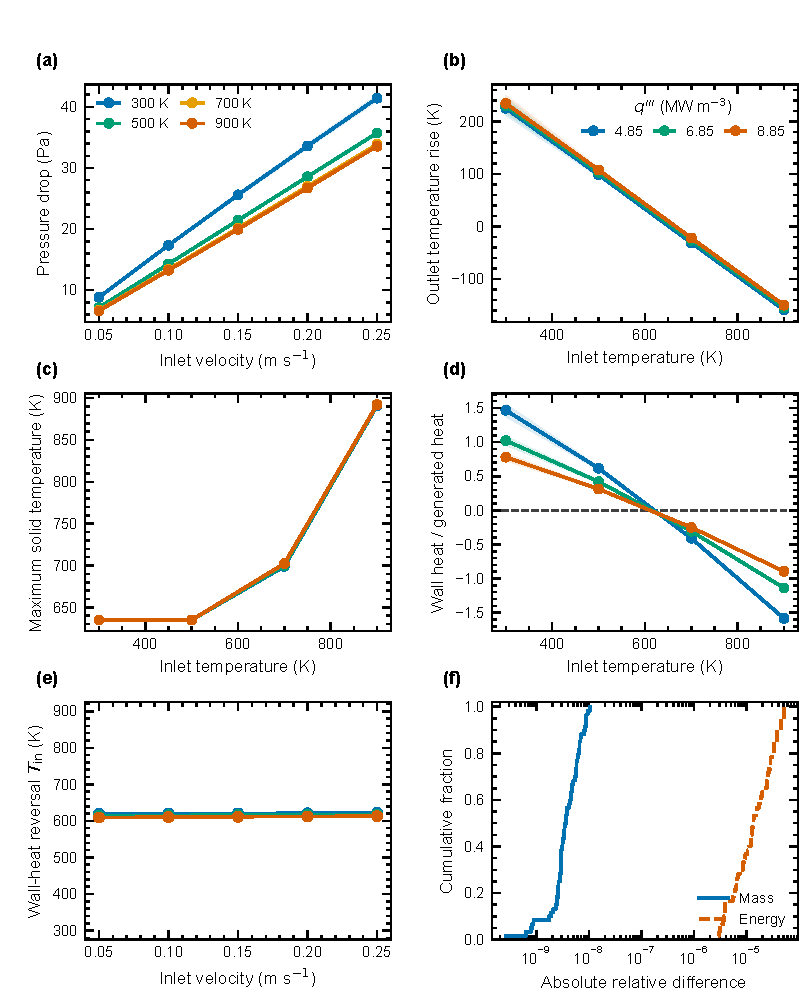
\includegraphics[width=\textwidth,height=0.75\textheight,keepaspectratio]{../figures/hccb_p418_physical_response.pdf}
\caption{Pore-resolved response across 60 conditions. (a) Pressure drop.
(b)--(d) Outlet-temperature rise, maximum solid temperature and normalized
signed wall heat; lines show medians and bands the sampled range.
(e) Inlet temperature at wall-heat reversal. (f) Mass and energy differences.}
\label{fig:physical_response}
\end{figure}
}{}

\IfFileExists{generated_steady_physics_text.tex}{%
\input{generated_steady_physics_text}}{}

\IfFileExists{generated_steady_final_windows.tex}{%
Across all 60 corrected-source-flow steady cases, the final 25 saved steady iterations changed the outlet temperature by at most \SI{0.0174}{K} and the maximum solid temperature by at most \SI{0.00212}{K}; among the 16 cases with paired full fields, the largest pointwise temperature change was \SI{0.0289}{K}.
}{}

\IfFileExists{generated_mesh_sensitivity.tex}{%
% Generated by code/build_hccb_p418_mesh_sensitivity_table.py
\begin{table*}[htbp]
\centering
\caption{Three-mesh sensitivity for the representative conjugate-heat-transfer condition. The equivalent cell size is $[(V_f+V_s)/(N_f+N_s)]^{1/3}$. Grid Convergence Index (GCI) values use the actual unequal refinement ratios and a safety factor of 1.25 \cite{celik2008gci}; no percentage GCI is reported for an oscillatory or unresolved sequence, or when the response crosses zero.}
\label{tab:mesh_sensitivity}
\small
\setlength{\tabcolsep}{4pt}
\resizebox{\textwidth}{!}{%
\begin{tabular}{@{}lrrrrrrr@{}}
\toprule
Grid & $N$ & $h_{\rm eq}$ ($\mu$m) & $\phi$ & $\Delta p$ (Pa) & $\Delta T_{\rm out}$ (K) & $\Delta T_{s,\max}$ (K) & $Q_{\rm wall}/Q_{\rm gen}$ \\
\midrule
Coarse & 361151 & 54.38 & 0.38591 & 23.3 & -26.52 & -0.1446 & -0.2733 \\
Medium & 947924 & 39.42 & 0.38661 & 25.64 & -26.2 & 0.05209 & -0.2942 \\
Fine & 1870064 & 31.43 & 0.38680 & 27 & -26.05 & 0.1608 & -0.3079 \\
\bottomrule
\end{tabular}
}
\par\vspace{0.5ex}
\resizebox{\textwidth}{!}{%
\begin{tabular}{@{}lrrr@{}}
\toprule
Quantity & Refinement behavior & Observed order & Fine-grid GCI \\
\midrule
Pressure drop & monotonic & 0.692 & 37.153\% \\
Outlet temperature rise & monotonic & 1.387 & 1.962\% \\
Maximum solid-temperature change & near-zero sign change & -- & -- \\
Signed wall heat / generated power & monotonic & 0.274 & 86.657\% \\
\bottomrule
\end{tabular}
}
\end{table*}


The three-grid comparison separates integral thermal convergence from local
hydraulic and wall-heat sensitivity. The fine-grid GCI is 1.96\% for outlet
temperature change, but 37.2\% for pressure drop and 86.7\% for signed
cooling-wall heat fraction. The maximum-solid-temperature change is close to
zero and changes sign across the three grids, so a percentage GCI is not
reported for that quantity. The common fine mesh therefore supports the
temperature-field model comparison, while pressure loss and wall heat are
retained as explicitly mesh-sensitive observables.}{}

\IfFileExists{generated_scope_limits.tex}{%
A separate full-domain fluid mesh failed the ordinary \texttt{checkMesh} test, so no solver was run on that mesh and no full-domain result is claimed. This limitation is distinct from the accepted local three-grid sensitivity study reported above. On the accepted local mesh, fixed-flow medium-to-fine thermal-curve differences remained below 0.043\%. Three fully coupled Courant-number tests stopped between \SI{0.000468}{s} and \SI{0.001105}{s} after pressure left the helium-property range; a run with consistent inlet velocity and mass flux similarly reached \SI{93413.3}{Pa}, below its \SI{93900}{Pa} limit. Model claims therefore concern thermal evolution with a prescribed hydrodynamic field. A direct OpenFOAM implementation of the same helium transport correlations was verified pointwise without a flow solve. A matched-initial representative using that implementation advanced to \SI{0.001522}{s} before a solid heat-capacity query reached \SI{1308.8}{K}, above the registered \SI{1300}{K} limit~\cite{kleykamp1996enthalpy}; this startup is used only to delimit property validity, not as fully coupled accuracy evidence.
}{%
The fixed-flow time-step study gave maximum medium-to-fine thermal-curve
differences below 0.043\%. Fully coupled startup calculations left the
specified helium-property pressure range before \SI{0.002}{s}; the model
results therefore concern thermal evolution with a prescribed hydrodynamic
field.}

\IfFileExists{generated_final_uncertainty_text.tex}{%
\input{generated_final_uncertainty_text}}{}

\subsection{External consistency checks}

\IfFileExists{../figures/hccb_heat_ai_external_evidence.pdf}{%
\begin{figure}[!htbp]
\centering
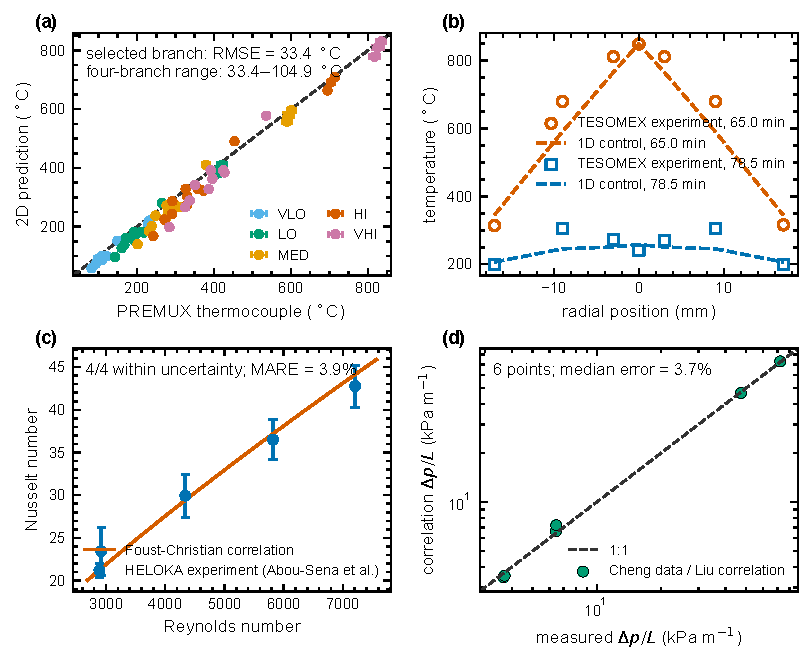
\includegraphics[width=\textwidth]{../figures/hccb_heat_ai_external_evidence.pdf}
\caption{External comparisons: (a) PREMUX thermocouples,
(b) TESOMEX radial temperatures, (c) HELOKA Nusselt numbers and (d) pressure
gradients in \SI{1}{mm} helium-cooled beds
\cite{hernandez2017premux,mohammed2018tesomex,abousena2023hcpb,
cheng2024pressure,liu2024unitary}. The data are not training labels.}
\label{fig:external_evidence}
\end{figure}
}{}

PREMUX and TESOMEX document spatial temperature structure that is not retained
by integral outlet measures. HELOKA and
fixed-bed data support the adopted convective and hydraulic scales, with mean
or median absolute relative errors of 3.9\% and 3.7\%, respectively. These
comparisons do not validate the specific three-dimensional packing.

\subsection{Sensitivity to pebble arrangement}

Nine matched conditions were recalculated on an independently generated
spherical-pebble arrangement. Relative to the source arrangement, the absolute
change is at most 0.67\% for outlet temperature and 0.31\% for maximum solid
temperature, but 14.7--18.0\% for pressure drop. Thus the integral thermal
response is comparatively robust for these two arrangements, whereas the
hydraulic response remains strongly geometry dependent
(Fig.~\ref{fig:cross_packing_integral}).

\IfFileExists{../figures/hccb_p418_seed202_integral_9.pdf}{%
\begin{figure}[htbp]
\centering
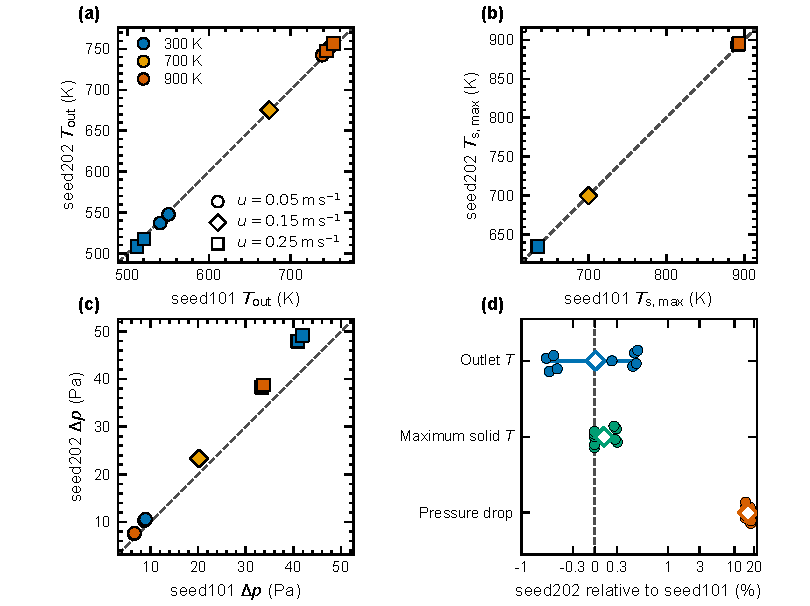
\includegraphics[width=\textwidth]{../figures/hccb_p418_seed202_integral_9.pdf}
\caption{Packing sensitivity at nine matched conditions. (a)--(c) Outlet
temperature, maximum solid temperature and pressure drop for seed101 and
seed202; the dashed line denotes parity, colors encode inlet temperature and
symbols encode inlet velocity. (d) Relative changes on a symmetric-logarithmic
axis (linear within $\pm1\%$); diamonds mark nine-condition means.
All points are direct calculations at the 200th steady nonlinear iteration.}
\label{fig:cross_packing_integral}
\end{figure}
}{}

\IfFileExists{generated_steady_model_comparison_validated.tex}{%
\subsection{Prediction of unseen steady conditions}
\IfFileExists{../figures/hccb_p418_steady_model_comparison.pdf}{%
\begin{figure}[!t]
\centering
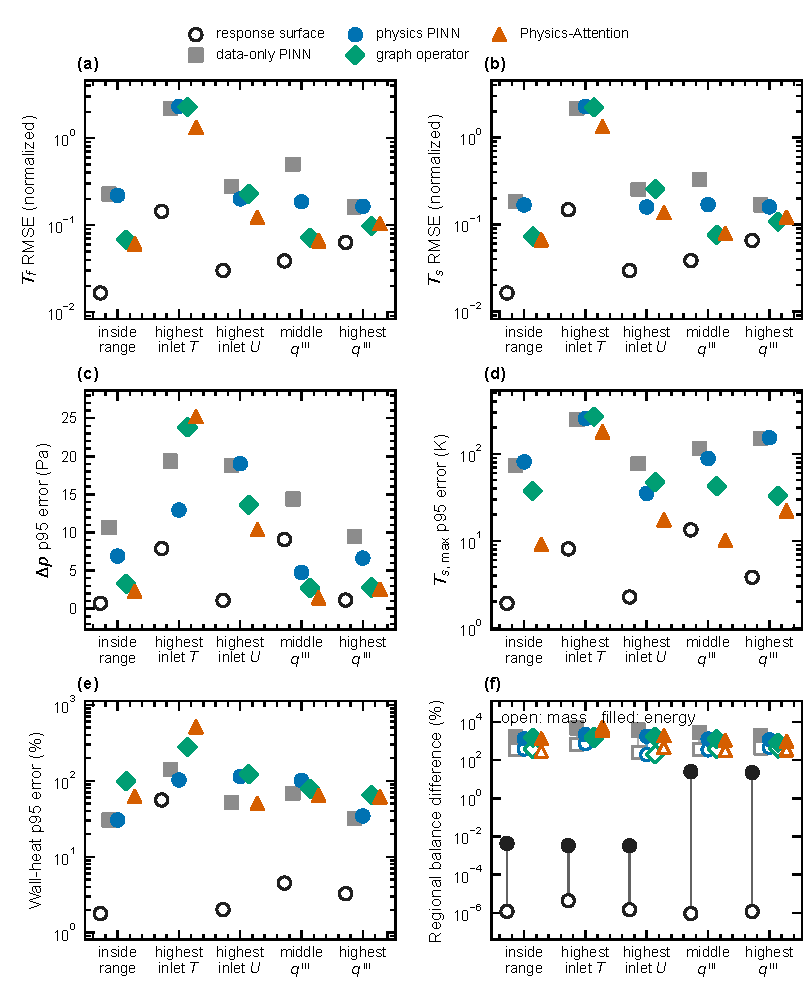
\includegraphics[width=\textwidth,height=0.75\textheight,keepaspectratio]{../figures/hccb_p418_steady_model_comparison.pdf}
\caption{Steady prediction on five complete-condition splits. Response-surface,
PINN, graph-operator and Physics-Attention models use identical temperature,
pressure, wall-heat and finite-volume balance measures.}
\label{fig:steady_model_comparison}
\end{figure}
}{}

\IfFileExists{generated_steady_performance.tex}{%
\begin{table*}[htbp]
\centering
\scriptsize
\setlength{\tabcolsep}{1.8pt}
\caption{Steady prediction accuracy and computational cost. Accuracy entries are the worst values across the five complete-condition splits in Figure~\ref{fig:steady_model_comparison}. Training and inference times are medians across the same five runs. The response-surface parameter range reflects validation-based selection between its linear and quadratic bases; neural-network parameter counts are fixed across splits. Times are measured values from the recorded computing device for each method and are not normalized to identical hardware.}
\label{tab:steady_performance}
\begin{tabular*}{\textwidth}{@{\extracolsep{\fill}}lrrrrrrr@{}}
\toprule
Method & \shortstack{Solid-$T$\\nRMSE} & \shortstack{Max-$T$ p95\\(K)} & \shortstack{Wall-heat p95\\(\%)} & \shortstack{Energy diff.\\(\%)} & \shortstack{Params\\(M; range)} & \shortstack{Train\\(min)} & \shortstack{Infer\\(ms)} \\
\midrule
response surface & 0.148 & 13.4 & 55.9 & 25 & 1.67--4.16 & 0.185 & 0.825 \\
data-only PINN & 2.17 & 246 & 140 & 4.89e+03 & 0.0368 & 0.878 & 4.93 \\
physics PINN & 2.27 & 253 & 114 & 2.2e+03 & 0.0368 & 0.898 & 5.14 \\
graph operator & 2.22 & 266 & 279 & 1.73e+03 & 1.45 & 20.7 & 116 \\
Physics-Attention & 1.33 & 178 & 510 & 5.41e+03 & 2.61 & 13.8 & 71.6 \\
\bottomrule
\end{tabular*}
\end{table*}
}{}
\IfFileExists{generated_steady_result_text.tex}{%
Across the five complete-condition splits, the lowest worst-case values for the six separately evaluated quantities are fluid-temperature nRMSE 0.144, solid-temperature nRMSE 0.148, pressure p95 error 9.07~Pa, solid maximum-$T$ p95 error 13.4~K, wall-heat p95 error 55.9~\%, regional energy difference 25~\%. All six are produced by the response surface; the separate quantities are not combined into a scalar model score.

With identical coordinate-network form, initialization, observations and optimization schedule, the data-only and physics-informed PINNs give, respectively, solid-temperature nRMSE 2.17 versus 2.27, wall-heat p95 error 140~\% versus 114~\%, regional energy difference 4.89e+03~\% versus 2.2e+03~\%. This paired comparison isolates the effect of the finite-volume mass, energy and interface-flux terms; all independent-condition values remain in Figure~\ref{fig:steady_model_comparison}.

The temperature-extrapolation split comprises training 30 conditions (30 wall-to-fluid, 0 fluid-to-wall), validation 15 conditions (0 wall-to-fluid, 15 fluid-to-wall), independent prediction 15 conditions (0 wall-to-fluid, 15 fluid-to-wall). It therefore measures transfer across the signed wall-heat change, not only interpolation between nearby inlet temperatures. The interleaved independent set contains 12 conditions (6 wall-to-fluid, 6 fluid-to-wall).

The two heat-source splits contain one training source level, so its zero-variance input is zero in every role; they test stability at unseen source levels, not learned source sensitivity.
}{}
\IfFileExists{generated_steady_seed_robustness_text.tex}{%
Across three independent initializations on the registered main split, the 
Transolver gives a solid-temperature nRMSE of $0.0675 \pm 0.0026$ and a maximum-solid-temperature p95 error of $11.9 \pm 1.2$~K.  The corresponding graph-operator values are $0.0725 \pm 0.0014$ and $27.1 \pm 8.9$~K.
This repeatability in temperature does not imply local energy closure: the Transolver wall-heat p95 error is $73.5 \pm 31.8$\%, and its mean regional energy-difference measure is $1321 \pm 63$\%.  The latter quantities are therefore retained as separate acceptance measures rather than being inferred from temperature accuracy.
}{}
}{}

\subsection{Prediction of held-out thermal trajectories}

Complete trajectories, rather than isolated time points, are withheld from
training and model selection. Persistence, DMDc, POD correction, diffusion
refinement and data-only or physics-constrained graph--Transformers are tested
on the same four endpoint pairs. Two temperature steps also withhold both
steady endpoints, testing the complete frozen steady-to-transient chain.

\IfFileExists{generated_transient_model_comparison_validated.tex}{}{%
\IfFileExists{generated_regional_dynamics_text.tex}{%
On the strict endpoint-pair holdout, repeating the initial temperature field gave fluid- and solid-temperature RMSE values of 3.63 and 3.55\,K, whereas continuous-time regional DMDc gave 5.45 and 5.03\,K. The lowest solid-field error was obtained by Initial-field persistence (3.55\,K), whereas the lowest hotspot p95 displacement was obtained by Initial-field persistence (2.48\,mm). These quantities are reported separately because a lower field-average temperature error does not by itself prove more accurate hotspot localization.
}{}
}

\IfFileExists{generated_transient_model_comparison_validated.tex}{%
\IfFileExists{../figures/hccb_p418_transient_model_comparison.pdf}{%
\begin{figure}[!htbp]
\centering
\includegraphics[width=\textwidth,height=0.75\textheight,keepaspectratio]{../figures/hccb_p418_transient_model_comparison.pdf}
\caption{Held-out thermal-trajectory prediction after validation-only model
and loss-weight selection. Solid-temperature responses to (a) velocity
increase, (b) velocity decrease, (c) heat-source increase and (d) heat-source
decrease. (e) Temperature error versus finite-volume energy-equation RMSE
after projection onto the common regional basis. (f) Accuracy versus
complete-chain speed-up relative to 32-rank \OpenFOAM{}; training and
data-generation costs are reported separately.}
\label{fig:transient_model_comparison}
\end{figure}
}{}
}{}

% The validated marker below supplies these values.  Empty fallbacks keep old
% preview metrics out of the manuscript source and are never typeset without
% that marker.
\providecommand{\PFieldModelLabel}{}
\providecommand{\PFieldFluidRMSE}{}
\providecommand{\PFieldSolidRMSE}{}
\providecommand{\PFieldFluidMaxError}{}
\providecommand{\PFieldSolidMaxError}{}
\IfFileExists{generated_openfoam_model_field_comparison_validated.tex}{%
\input{generated_openfoam_model_field_comparison_validated}
\IfFileExists{../figures/hccb_p418_openfoam_model_field_comparison.pdf}{%
\begin{figure}[!htbp]
\centering
\includegraphics[width=\textwidth,height=0.76\textheight,keepaspectratio]{../figures/hccb_p418_openfoam_model_field_comparison.pdf}
\caption{Regionalized OpenFOAM--model temperatures at \SI{25}{s} for an
independent test heat-source increase; the model was selected using validation trajectories only.
Rows: reference, \PFieldModelLabel{} prediction and
signed error; columns: fluid and solid phases. Reference and prediction
share a scale. Error colors are clipped at the 99th percentile; annotated
extrema and metrics are unclipped. Section interpolation is visual only;
metrics use the original regional nodes.}
\label{fig:field_cloud_comparison}
\end{figure}

The full regional-field fluid/solid RMSE in
Fig.~\ref{fig:field_cloud_comparison} is
\SI{\PFieldFluidRMSE}{K}/\SI{\PFieldSolidRMSE}{K}, and the corresponding
maximum absolute errors are \SI{\PFieldFluidMaxError}{K} and
\SI{\PFieldSolidMaxError}{K}.  These maxima are reported without color-scale
clipping, so the figure distinguishes representative spatial fidelity from
isolated extreme errors rather than reporting only an averaged score.
}{}
}{}

\IfFileExists{generated_transient_performance.tex}{%
\input{generated_transient_performance}}{}
\IfFileExists{generated_transient_result_text.tex}{%
\input{generated_transient_result_text}}{}
\IfFileExists{generated_fused_chain_text.tex}{%

\input{generated_fused_chain_text}}{}
\IfFileExists{generated_high_re_comparison.tex}{%
The three frozen graph--Transformer variants were additionally evaluated on
six independent high-velocity histories that were excluded from training,
normalization and model selection.  Their aggregate fluid/solid temperature
RMSE values are 122.6--\SI{123.9}{K} and
116.2--\SI{117.7}{K}, respectively; the fixed-weight physical residuals
do not improve this transfer.  Source steps remain within \SIrange{3.2}{6.3}{K}
and velocity steps within \SIrange{14.8}{21.0}{K}, whereas temperature steps
produce \SIrange{198.8}{215.9}{K}.  The dominant limitation is therefore
temperature-range extrapolation rather than flow-rate transfer alone.}{}

\subsection{Model value and scope}

\IfFileExists{generated_final_discussion.tex}{\input{generated_final_discussion}}{%
The comparison first quantifies the native-cell temperature structure lost by
regionalization. It then tests physical constraints, graph attention and
diffusion refinement against data-only, response-surface, coordinate-PINN,
DMDc and low-rank alternatives. All methods use identical condition splits,
field targets and conservation measures; complexity is justified only by an
improvement on these common tests.

For the 60 steady conditions, a low-dimensional response surface is more
robust than the neural models for integral quantities. On six independent
high-velocity histories, three frozen graph--Transformer variants have similar
temperature errors, and fixed-weight mass, energy and interface-flux residuals
do not improve transfer. The main failure is the large inlet-temperature step,
not the heat-source or flow-rate step. Physical residuals are therefore used
as conservation diagnostics, not as proof that a constrained network must be
more accurate.

The fixed-flow trajectories exclude initial hydrodynamic adjustment, and a
local crop with two packings cannot establish component-scale performance.
The independent-packing test uses intact spheres without particle-contact conduction. Contact
conduction under stress and rarefied gas transport affect compressed or
low-pressure beds
\cite{moscardini2018tdem,peeketi2018compacted,desu2020tdem}, but lie outside
the present model. Nor does it replace thermo-mechanical analyses of contacts,
size redistribution and spatial crushing \cite{wang2026crushable}. A
blanket-module extension requires its nuclear
heating field, geometry, boundaries and contact or gap conductances.
}

\section{Conclusions}

\IfFileExists{generated_final_conclusions.tex}{\input{generated_final_conclusions}}{%
We compare PINN, graph--Transformer and diffusion-refinement models against
finite-volume reference data for internally heated
solid-breeder pebble beds. The reference set contains 60 steady conditions and
12 fixed-flow thermal steps. Nine matched calculations on an independent
spherical packing show similar outlet and maximum-solid temperatures but a
strongly packing-dependent pressure drop. A transferable thermal operator
therefore still requires packing-specific hydraulic information. The
fixed-flow histories exclude the initial fully coupled response, while the
failed full-domain mesh and property-range tests are reported only as limits.
The present evidence does not by itself establish a final model ranking.
}

\section*{Data and code availability}

The source code, parameter tables, processed figure data, result summaries and
recorded software versions are available at
\url{https://github.com/wangjianfttt/fusion-pebble-bed-heat-transfer-ai}.
Original code is released under the MIT License, and processed numerical data
and figure tables are released under CC BY 4.0. The repository includes a
compact archive for reproducing the reported response, independent-packing and
model-comparison figures. The larger decomposed \OpenFOAM{} fields are retained
in the institutional archive because of their size and are available from the
corresponding author on reasonable request. A versioned DOI will be added to
the repository record before submission.

\section*{CRediT authorship contribution statement}

\textbf{Jian Wang:} Conceptualization, Methodology, Software, Investigation, Formal analysis, Visualization, Writing -- original draft.
\textbf{Wei Wen:} Data curation, Visualization, Writing -- review and editing.
\textbf{Gang Shen:} Methodology, Project administration, Writing -- review and editing.
\textbf{Mingzhun Lei:} Methodology, Writing -- review and editing.
\textbf{Yuntao Song:} Supervision, Project administration, Writing -- review and editing.

\section*{Declaration of competing interest}

The authors declare that they have no known competing financial interests or personal relationships that could have appeared to influence the work reported in this paper.

\section*{Declaration of generative AI and AI-assisted technologies in the manuscript preparation process}

During the preparation of this work, the authors used OpenAI Codex for language revision, code review and workflow assistance. The authors independently verified the calculations, data, citations and final text, reviewed and edited all AI-assisted content, and take full responsibility for the content of the article. No generative AI system was used to create or alter the scientific images or numerical results.

\section*{Acknowledgements}

This work was supported by the Anhui Provincial Natural Science Foundation (2408085QA030), project No. 2504000000-04-05-42671, the Anhui Intelligent Mine Technology and Equipment Engineering Research Center (AIMTEERC202307), the Science Foundation of the Institute of Plasma Physics, Chinese Academy of Sciences (DSJJ-2025-08), and the China Postdoctoral Science Foundation under Grant No. 2024M753266.

\begingroup
\small
\bibliographystyle{elsarticle-num}
\bibliography{references}
\endgroup

\end{document}
